\documentclass[10pt,presentation,shownotes]{beamer}
\usetheme{Warsaw}
\usecolortheme{dove}

\beamertemplatenavigationsymbolsempty

\usepackage{beamerthemesplit}
\usefonttheme{default}
\setbeamertemplate{caption}[numbered]
\setbeamercolor{block body example}{bg=green!12}
% \setbeamertemplate{navigation symbols}{}
% \setbeamercovered{transparent}
\setbeamertemplate{theorems}[numbered]

\usepackage[utf8]{inputenc}
\usepackage[T1]{fontenc}
\usepackage{lmodern}
\usepackage[english]{babel}
\usepackage{csquotes}
\usepackage{mathtools,amsfonts,amssymb,tikz-cd,hyperref,caption,pstricks,setspace,booktabs,hyperref}
\usepackage{appendixnumberbeamer}
\usepackage{xcolor}
\hypersetup{
	colorlinks,
	linkcolor={blue!50!black},
	citecolor={blue!50!black},
	urlcolor={blue!80!black}
}

% We use BiBLaTeX for our bibliography.
% \usepackage[backend=biber,style=alphabetic]{biblatex}
% \renewcommand*{\nameyeardelim}{\addcomma\addspace}

% \addbibresource{References/ref.bib}

\makeatletter
\def\th@remark{%
    \normalfont % body font
    \setbeamercolor{block title example}{bg=orange,fg=black}
    \setbeamercolor{block body example}{bg=orange!20,fg=black}
    \def\inserttheoremblockenv{exampleblock}
  }
\makeatother

\theoremstyle{remark}
\newtheorem*{remark}{Remark}

\setbeamertemplate{headline}
{
  \leavevmode%
  \hbox{%
  \begin{beamercolorbox}[wd=.5\paperwidth,ht=2.5ex,dp=1ex,left,leftskip=1em]{section in head/foot}%
    \usebeamerfont{subsection in head/foot}\hspace*{2ex}\insertshorttitle
  \end{beamercolorbox}%
  \begin{beamercolorbox}[wd=.5\paperwidth,ht=2.5ex,dp=1ex,center]{date in head/foot}%
    \usebeamerfont{date in head/foot}\insertshortdate{}\hspace*{2ex}
  \end{beamercolorbox}}%
  \vskip0pt%
}

\makeatletter
\setbeamertemplate{footline}
{
  \leavevmode%
  \hbox{%
  \begin{beamercolorbox}[wd=.33\paperwidth,ht=2.25ex,dp=1ex,center]{author in head/foot}%
    \usebeamerfont{author in head/foot}\insertshortauthor~~\beamer@ifempty{\insertshortinstitute}{}{(\insertshortinstitute)}
  \end{beamercolorbox}%
  \begin{beamercolorbox}[wd=.34\paperwidth,ht=2.25ex,dp=1ex,center]{subsection in head/foot}%
    \usebeamerfont{section in head/foot}\hspace*{1ex}\insertsectionhead\hspace*{1ex}
  \end{beamercolorbox}%
  \begin{beamercolorbox}[wd=.33\paperwidth,ht=2.25ex,dp=1ex,right, rightskip=1em]{section in head/foot}%
    \usebeamerfont{section in head/foot}\insertsubsectionhead\hspace*{2ex}
  \end{beamercolorbox}}%
  \vskip0pt%
}
\makeatother

\makeatletter
\setbeamertemplate{frametitle}{
    \ifbeamercolorempty[bg]{frametitle}{}{\nointerlineskip}%
    \@tempdima=\textwidth%
    \advance\@tempdima by\beamer@leftmargin%
    \advance\@tempdima by\beamer@rightmargin%
    \begin{beamercolorbox}[sep=0.3cm,center,wd=\the\@tempdima]{frametitle}
        \usebeamerfont{frametitle}%
        \vbox{}\vskip-1ex%
        \if@tempswa\else\csname beamer@ftecenter\endcsname\fi%
        \strut\insertframetitle\strut\par%
        {%
            \ifx\insertframesubtitle\@empty%
            \else%
            {\usebeamerfont{framesubtitle}\usebeamercolor[fg]{framesubtitle}\insertframesubtitle\strut\par}%
            \fi
        }%
        \vskip-1ex%
        \if@tempswa\else\vskip-.3cm\fi% set inside beamercolorbox... evil here...
    \end{beamercolorbox}%
}
\makeatother

% This code displays an updating ToC at the beginning of every section.
\AtBeginSection[]
{
	\begin{frame}
	\frametitle{Table of Contents}
	\tableofcontents[currentsection]
	\end{frame}
}

\makeatletter
\newcommand<>{\insertsubsectiontitle}{\frametitle{\insertsubsection}}
\let\oldbeamer@checkframetitle\beamer@checkframetitle% Store the \frametitle checking mechanism
\renewcommand<>{\subsection}{%
  \gdef\beamer@checkframetitle{% Update \frametitle checking to ...
    \insertsubsectiontitle% ...insert the section title and...
    \global\let\beamer@checkframetitle\oldbeamer@checkframetitle% ...revert to it's old definition
  }% Regular \section stuff follows
  \alt#1{\@ifnextchar[\beamer@subsection\beamer@@subsection}
    {\beamer@secgobble}}
\makeatother

\makeatletter
\newenvironment<>{proofs}[1][\proofname]{%
    \par
    \def\insertproofname{#1\@addpunct{.}}%
    \usebeamertemplate{proof begin}#2}
  {\usebeamertemplate{proof end}}
\makeatother

\title[Problemas de S-L e o método do tiro
\hspace{0.3cm}\insertframenumber/\inserttotalframenumber
]
{Problemas de Sturm-Liouville e o método do tiro}
\author[Caio Tomás]{Caio Tomás de Paula \\
Professor: Yuri Dumaresq Sobral}
\date[Introdução a Métodos Computacionais em EDOs -- 14/02]{Introdução a Métodos Computacionais em EDOs}
\institute[MAT -- UnB]{Universidade de Brasília \\ Departamento de Matemática}
% \titlegraphic{\includegraphics[width=1\textwidth]{Colorida.png}}

\usepackage{tikz}
\usepackage{amsmath}
\usepackage{verbatim}
\usetikzlibrary{arrows,shapes}

\tikzstyle{terminator} = [rectangle, draw, text centered, rounded corners, minimum height=2em]
\tikzstyle{process} = [rectangle, draw, text centered, minimum height=2em]
\tikzstyle{decision} = [diamond, draw, text centered, minimum height=2em]
\tikzstyle{data}=[trapezium, draw, text centered, trapezium left angle=60, trapezium right angle=120, minimum height=2em]
\tikzstyle{connector} = [draw, -latex']

\newcommand{\C}{\mathbb{C}}
\newcommand{\R}{\mathbb{R}}
\newcommand{\N}{\mathbb{N}}
\newcommand{\Z}{\mathbb{Z}}

\newcommand*\diff{\mathop{}\!\mathrm{d}}

% \usepackage{multimedia}
% \input{embed_video}

\newcommand{\hiddencell}[2]{\action<#1->{#2}}

\begin{document}

\maketitle

% For every picture that defines or uses external nodes, you'll have to
% apply the 'remember picture' style. To avoid some typing, we'll apply
% the style to all pictures.
\tikzstyle{every picture}+=[remember picture]

% By default all math in TikZ nodes are set in inline mode. Change this to
% displaystyle so that we don't get small fractions.
\everymath{\displaystyle}
%

%
\begin{frame}{Qual é o problema?}
    Um problema de Sturm-Liouville regular tem a forma
    \tikzstyle{na} = [baseline=-.5ex]
    %
    \begin{itemize}[<+-| alert@+>]
        \item Peso
            \tikz[na]\node [coordinate] (n1) {};
    \end{itemize}
    %
    %
    \begin{equation*}
    \tag{S-L regular}
        \left\{
        \begin{array}{l}
            -(p(x)y')' + q(x)y 
            = \textcolor{red}{\lambda}\tikz[baseline]{
                \node[fill=red!20,anchor=base] (t1)
                {$r(x)$};   
            }y, \, a \leq x \leq b \\[0.2cm]
            \tikz[baseline]{
                \node[fill=blue!20,anchor=base] (t2)
                {$\alpha y(a) + \beta y'(a) = 0$};   
            } \\[0.2cm]
            \tikz[baseline]{
                \node[fill=green!20,anchor=base] (t3)
                {$\gamma y(b) + \delta y'(b) = 0$};   
            }
        \end{array}
        \right.
    \end{equation*}
    %
    \begin{itemize}[<+-| alert@+>]
        \item Condições de contorno
            \tikz[na]\node [coordinate] (n2) {};
        % \item Condição de contorno
        %     \tikz[na]\node [coordinate] (n3) {};
    \end{itemize}
    %
    \begin{tikzpicture}[overlay]
        \path[->]<1-> (n1) edge [out=0, in=135] (t1);
        \path[->]<2-> (n2) edge [out=0, in=-5] (t2);
        \path[->]<3-> (n2) edge [out=0, in=-10] (t3);
    \end{tikzpicture}
    %
    \pause com
    \begin{itemize}
        \item $p, q > 0$ em $[a,b]$;
        \item $p, q, r\in C^2([a,b])$;
        \item $\alpha, \beta, \gamma, \delta \in\R$ com $|\alpha| + |\beta| > 0$
        e $|\gamma| + |\delta| > 0$;
    \end{itemize}
\end{frame}
%

%
\begin{frame}{Resultados fundamentais}
    \begin{itemize}
        \item Estes problemas são abundantes em problemas de EDPs lineares separáveis, como
        %
        \begin{itemize}
            \item eq. do calor;
            \item eq. da onda;
            \item eq. de Laplace/Poisson.
        \end{itemize} \pause
        %
        \item os autovalores são reais e podem ser ordenados,
        %
        \[
            0 < \lambda_1 < \lambda_2 < \cdots < \lambda_n < \cdots \to \infty.
        \] \pause
        %
        \item a cada autovalor $\lambda_n$ está associada uma única (a menos
        de multiplicação por escalar) autofunção $y_n$, que tem exatamente 
        $n-1$ zeros em $(a,b)$, chamada \textbf{$n$-ésima solução fundamental}. \pause
    
        \item as autofunções (normalizadas) formam uma base ortonormal com
        respeito ao produto interno de peso $r$,i.e.,
        %
        \[
            \left\langle y_n, y_m \right\rangle
            = \int_a^b y_n(x)y_m(x)r(x) \diff x
            = \delta_{mn}.
        \]
        %
    \end{itemize}
    %
\end{frame}
%

%
\begin{frame}{Qual é o método?}
    Dado o PVC
    %
    \begin{equation*}
        \left\{
        \begin{array}{l}
            -(p(x)y')' + q(x)y 
            = \lambda r(x)y, \, a \leq x \leq b \\[0.1cm]
            \alpha y(a) + \beta y'(a) = 0   
             \\[0.1cm]
            \gamma y(b) + \delta y'(b) = 0
        \end{array}
        \right.
    \end{equation*} \pause
    %
    geramos o PVI
    %
    \begin{equation*}
        \left\{
            \begin{array}{l}
                -(p(x)u')' + (q(x) - \lambda r(x))u = 0, \, a \leq x \leq b \\[0.1cm]
                u(a) = -\beta/\sqrt{\alpha^2 + \beta^2}, \\[0.1cm]
                u'(a) = \alpha/\sqrt{\alpha^2 + \beta^2}.
            \end{array}
        \right.
    \end{equation*} \pause
    %
    Pela simplicidade dos autovalores e unicidade das autofunções,
    segue que a única autofunção (normalizada) associada a cada autovalor é tal que
    %
    \[
        y(a) = -\beta/\sqrt{\alpha^2 + \beta^2}, \quad
        y'(a) = \alpha/\sqrt{\alpha^2 + \beta^2}.
    \] \pause
    %
    Resolver o  PVC $\iff$ resolver o PVI 
    e encontrar a raiz de
    %
    \begin{equation*}
        \boxed{F(\lambda) = \gamma u(b, \lambda) + \delta u'(b, \lambda).}
    \end{equation*}
    %
\end{frame}
%

%
\begin{frame}{Qual é o método?}
    \begin{center}
    \begin{tikzpicture}[node distance = 2cm, scale=0.9]
        % \node [terminator, fill=blue!20] (start) {\textbf{Inicialização das variáveis}};
        
        \node [process, fill=blue!20] at (0,-1.5) (PVI2) 
        {Resolver o PVI para $\lambda = \lambda_n^i$};
        
        \node [decision, fill=blue!20] at (0,-4.5) (decision)
        {$F(\lambda_n^i) < \mathrm{TOL}$?};
        
        \node [process, fill=red!20] at (4.5,-1.5) (chute) 
        {$\lambda_n^i \to \lambda_n^{i+1}$};
        
        \node [process, fill=green!20] at (0,-7.5) (encontrado)
        {Autovalor $\lambda_n$ encontrado!};
        
        \node [process, fill=blue!20] at (0,-9) (PVIFinal) 
        {Resolver o PVI para $\lambda = \lambda_n$};

        \node [terminator, fill=teal!20] at (-3.7,-4.5) (metodo)
        {RKE$4$};
        
        \node [data, fill=blue!20] at (5,-9) (salvamento) 
        {Salvar solução};
        
        % \node [terminator, fill=blue!20] at (0,-10.5) (end) {\textbf{Fim}};
        
        \node[draw=none] at (2.40, -4.25) (no) {Não};
        \node[draw=none] at (0.35, -6.70) (yes) {Sim};
        
        % \path [connector] (start) -- (PVI2);
        \path [connector] (PVI2) -- (decision);
        \path [connector] (decision) -| (chute);
        \path [connector] (decision) -- (encontrado);
        \path [connector] (chute) -- (PVI2);
        \path [connector] (metodo) |- (PVI2);
        \path [connector] (metodo) |- (PVIFinal);
        \path [connector] (encontrado) -- (PVIFinal);
        \path [connector] (PVIFinal) -- (salvamento);
        % \path [connector] (salvamento) -- (end);
    \end{tikzpicture}
\end{center}
    
\end{frame}
%

%
\begin{frame}{Câmbio, testando...}
    %
    \begin{tabular}{lc}
    \hiddencell{1}{
        \begin{tabular}{l}
            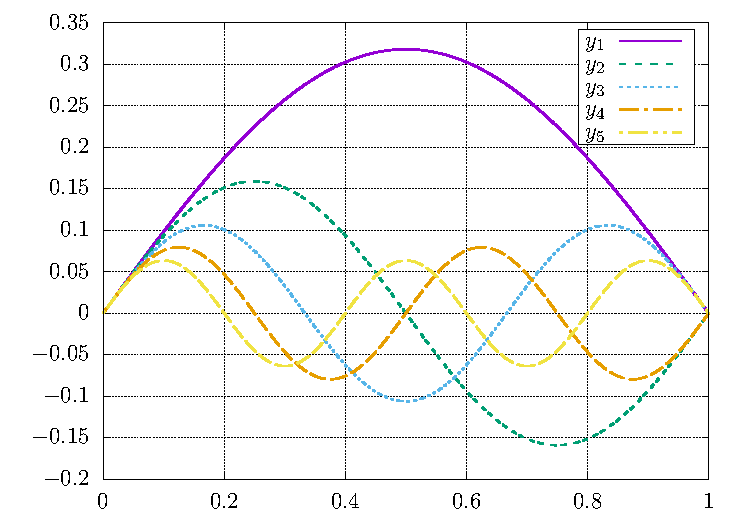
\includegraphics[width=0.45\textwidth]{Relatório/Figuras/FirstProblem.pdf}
        \end{tabular}
        }
        &
        \begin{tabular}{c}
            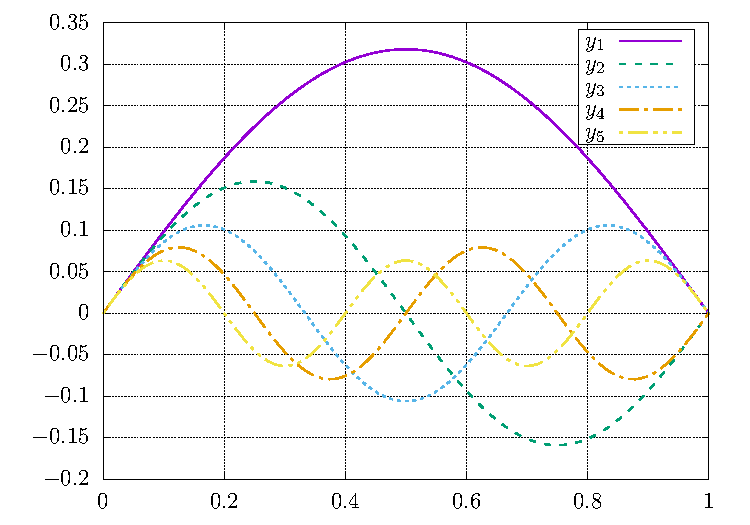
\includegraphics[width=0.45\textwidth]{Relatório/Figuras/FirstProblem_check.pdf}
        \end{tabular} \\
        \[
            \left\{
                \begin{array}{l}
                    y'' + \lambda y = 0, \, 0 \leq x \leq 1 \\[0.2cm]
                    y(0) = y(1) = 0,
                \end{array}
            \right.
        \] 
        & \resizebox{5.5cm}{!}{
        \begin{tabular}{cc|cc|c|c}
            % \hline
            % \multicolumn{2}{c}{Intervalo inicial} & \multicolumn{2}{c}{Autovalor encontrado}
            % & \multicolumn{2}{c}{} \\
            \hline
            $a$ & $b$ & $n$ & $\lambda_n$ & its. & \% erro \\
            \hline
            $-10000$ & $1000$ & $3$ & $88.82644$ & $35$ & $10^{-7}$ \\
            $-100$ & $1000$ & $9$ & $799.438$ & $28$ & $10^{-6}$ \\
            $-1$ & $2$ & --- & \textcolor{red}{$2$} & $\infty$ & --- \\
            $500$ & $30000$ & $54$ & $28780.16$ & $27$ & $10^{-3}$ \\
            $1$ & $3$ & --- & \textcolor{red}{$3$} & $\infty$ & --- \\
            $1$ & $10$ & $1$ & $9.869604$ & $24$ & $10^{-7}$ \\
            $-1000$ & $10$ & $1$ & $9.869604$ & $35$ & $10^{-7}$ \\
            \hline
        \end{tabular}
        } \\
        \[
            \lambda_n = n^2\pi^2, \quad y_n(x) = \sin(n\pi x)
        \]
        &
        %
    \end{tabular}
    %
\end{frame}
%

%
\begin{frame}{...e mais um problema regular...}

     %
    \begin{tabular}{cl}
    \begin{tabular}{l}
            \parbox{0.25\linewidth}{%  change the parbox width as appropiate
            \[
                \left\{
                    \begin{array}{l}
                        -y'' + xy = \lambda\cos(x)y, \\[0.1cm]
                        y(0) + y'(0) = 0 \\[0.1cm]
                        y(1) + y'(1) = 0.
                    \end{array}
                \right.
            \]
            }
        \end{tabular}
        &
    \hiddencell{1}{
        \begin{tabular}{c}
            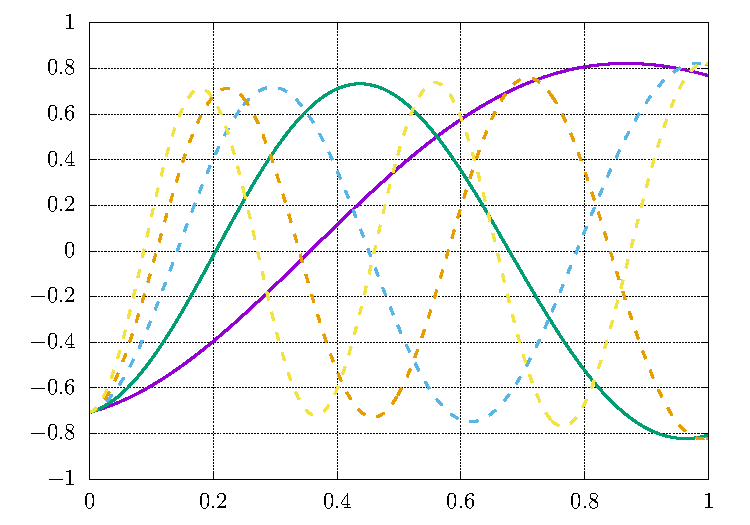
\includegraphics[width=0.65\textwidth]{Relatório/Figuras/SecondProblem.pdf}
        \end{tabular}
        }
        \\
    \end{tabular}
    %
    \centering
    \begin{tabular}{cc|cc|c}
        % \hline
        \multicolumn{2}{c}{Intervalo inicial} & \multicolumn{2}{c}{Autovalor encontrado} & \\
        \hline
        $a$ & $b$ & $n$ & $\lambda_n$ & \# iterações \\
        \hline
        $0$ & $15$ & $1$ & $13.57597859$ & $31$ \\
        $25$ & $60$ & $2$ & $49.200691955629736$ & $31$ \\
        $70$ & $120$ & $3$ & $108.32595458952710$ & $32$ \\
        $180$ & $240$ & $4$ & $191.05031406506896$ & $30$ \\
        $200$ & $350$ & $5$ & $297.39334740152117$ & $34$ \\
        \hline
    \end{tabular}
\end{frame}
%

%
\begin{frame}{...agora um problema singular...}
    Problemas de Sturm-Liouville singulares do \textcolor{red}{tipo I} são da forma
    %
    \begin{equation*}
        \left\{
        \begin{array}{l}
            -(p(x)y')' + q(x)y = \lambda r(x)y, \, a < x < b \\[0.2cm]
            |y(a)| < \infty \\[0.2cm]
            \gamma y(b) + \delta y'(b) = 0, \, |\gamma| + |\delta| \neq 0.
        \end{array}
        \right.
    \end{equation*}
    %
    com
    %
    \begin{itemize}
        \item $p(x) \geq 0$ seja contínuo em $[a,b]$, diferenciável em $a$, não nulo em $(a,b]$
        e tal que $p(a) = 0$ e $p'(a) \neq 0$;
        \item $q\in C^1([a,b])$;
        \item $p,q$ funções reais e $\gamma, \delta\in\R$;
        \item $r\in C^1([a,b])$ e ou $r(x) > 0$ em $[a,b]$ ou $r(x) = (x-a)^m\rho(x)$
        com $m>0$ e $\rho(x) > 0$ contínua em $[a,b]$.
    \end{itemize}
    %
\end{frame}
%

%
\begin{frame}{Qual é o método?}
    Dado o PVC
    %
    \begin{equation*}
        \left\{
        \begin{array}{l}
            -(p(x)y')' + q(x)y = \lambda r(x)y, \, a < x < b \\[0.2cm]
            |y(a)| < \infty \\[0.2cm]
            \gamma y(b) + \delta y'(b) = 0, \, |\gamma| + |\delta| \neq 0.
        \end{array}
        \right.
    \end{equation*}
    %
    geramos o PVI
    %
    \begin{equation*}
        \left\{
            \begin{array}{l}
                -(p(x)u')' + (q(x) - \lambda r(x))u = 0, \, a \leq x\leq b \\[0.1cm]
                u(a) = 1, \\[0.1cm]
                u'(a) = (q(a) - \lambda r(a))/p'(a)
            \end{array}
        \right.
    \end{equation*}
    %
    Resolver o  PVC $\iff$ resolver o PVI 
    e encontrar a raiz de
    %
    \begin{equation*}
        \boxed{F(\lambda) = \gamma u(b, \lambda) + \delta u'(b, \lambda).}
    \end{equation*}
    %
\end{frame}
%

%
\begin{frame}{...agora um problema singular...}
    Vamos resolver, como exemplo,
    %
    \[
        \left\{
        \begin{array}{l}
            -(xy')' = \lambda xy, \, 0 \leq x\leq 1 \\[0.1cm]
            |y(0)| < \infty, \\[0.1cm]
            \gamma y(1) + \delta y'(1) = 0,
        \end{array}
    \right.
    \] \pause
    %
    As autofunções são dadas por
    %
    \[
        y_n(x) = J_0\left(\sqrt{\lambda_n}x\right), \, n = 1, 2, \dots,
    \]
    %
    com $\lambda_n$ raízes de
    %
    \[
        F(\lambda) = J_0\left(\sqrt{\lambda}\right) + \sqrt{\lambda}J_0'\left(\sqrt{\lambda}\right)
                   = J_0\left(\sqrt{\lambda}\right) - \sqrt{\lambda}J_1\left(\sqrt{\lambda}\right).
    \] \pause
    %
    O PVI associado para o método do tiro é, portanto,
    %
    \[
        \left\{
            \begin{array}{l}
                -(xu')' = \lambda xu, \, 0 \leq x\leq 1 \\[0.1cm]
                u(a) = 1, \\[0.1cm]
                u'(a) = 0.
            \end{array}
        \right.
    \]
    %
\end{frame}
%

%
\begin{frame}{...agora um problema singular...}
    \centering
    \begin{tabular}{cc|cc|c}
        % \hline
        \multicolumn{2}{c}{Intervalo inicial} & \multicolumn{2}{c}{Autovalor encontrado} & \\
        \hline
        $a$ & $b$ & $n$ & $\lambda_n$ & \# iterações \\
        \hline
        $1$ & $12$ & $1$ & $1.5769950870890170$ & $32$ \\
        $10$ & $25$ & $2$ & $16.642215733882040$ & $31$ \\
        $47$ & $67$ & $3$ & $51.205829855054617$ & $30$ \\
        $87$ & $125$ & $4$ & $105.49412574432790$ & $30$ \\
        $150$ & $200$ & $5$ & $179.51907205861062$ & $31$ \\
        \hline
    \end{tabular}
    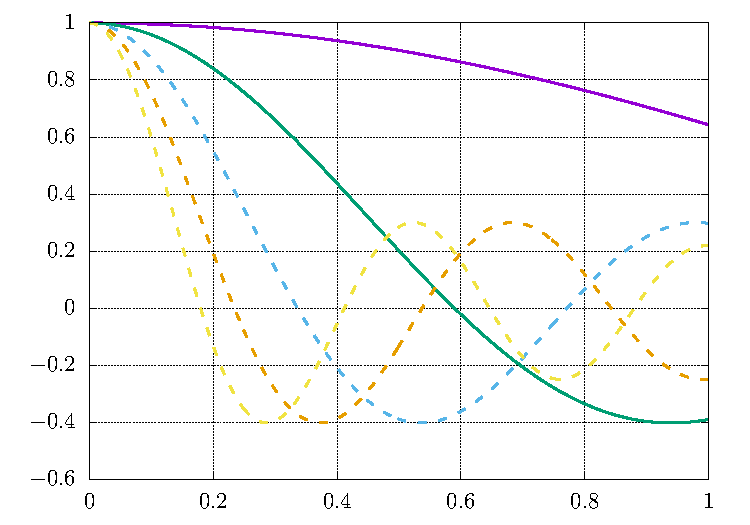
\includegraphics[width=.7\textwidth]{Relatório/Figuras/SingularProblem.pdf}
\end{frame}
%

%
\begin{frame}{...e mais um problema singular!}
    %
    \begin{tabular}{cl}
    \begin{tabular}{l}
            \parbox{0.25\linewidth}{%  change the parbox width as appropiate
            \[
                \left\{
            \begin{array}{l}
                -(gxX')' = \lambda X, \, \\[0.1cm]
                |X(0)| < \infty, \\[0.1cm]
                X(1) = 0,
            \end{array}
        \right.
            \]
            }
        \end{tabular}
        &
    \hiddencell{1}{
        \begin{tabular}{c}
            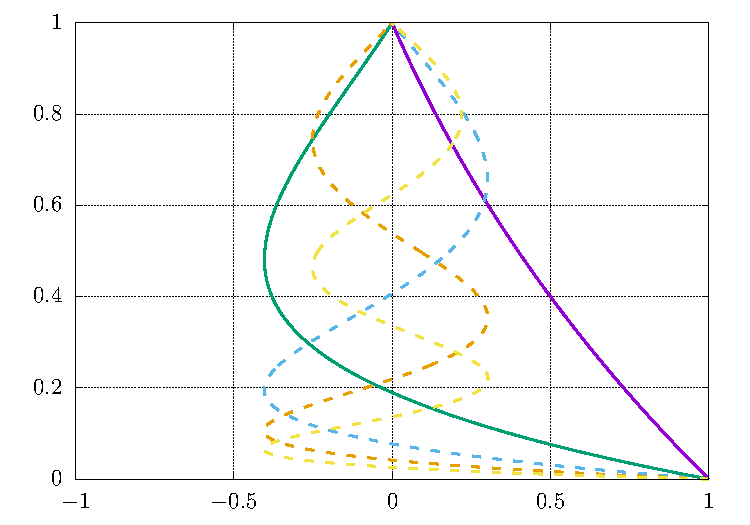
\includegraphics[width=0.65\textwidth]{Relatório/Figuras/CordaProblem.pdf}
        \end{tabular}
        }
        \\
    \end{tabular}
    %
    \centering
    \begin{tabular}{cc|cc|c}
        % \hline
        \multicolumn{2}{c}{Intervalo inicial} & \multicolumn{2}{c}{Autovalor encontrado} & \\
        \hline
        $a$ & $b$ & $n$ & $\lambda_n$ & \# iterações \\
        \hline
        $1$ & $20$ & $1$ & $14.168845105916262$ & $28$ \\
        $50$ & $80$ & $2$ & $74.656355008482933$ & $27$ \\
        $150$ & $200$ & $3$ & $183.48639830946922$ & $26$ \\
        $200$ & $350$ & $4$ & $340.69997835904360$ & $28$ \\
        $350$ & $800$ & $5$ & $546.32480936124921$ & $29$ \\
        \hline
    \end{tabular}
\end{frame}
%

\begin{frame}{Observações finais}
    %
    \begin{itemize}
        \item pode-se usar o método de Newton-Raphson para avançar nas estimativas
        dos autovalores: isso exige um palpite inicial mais consciente e resolver um segundo
        PVI, dado por (no caso regular)
        %
        \[
            \left\{
            \begin{array}{l}
                -(p(x)w')' + q(x)w = \lambda r(x)w, \, a \leq x \leq b \\[0.2cm]
                w(a) = 0, \\[0.2cm]
                w'(a) = 0.
            \end{array}
            \right.
        \]
        %
        cuja solução é tal que 
        \[
            \boxed{F'(\lambda) = \gamma w(b,\lambda) + \delta w'(b,\lambda);}
        \] \pause

        \item como o método do tiro é uma combinação de dois métodos (um para resolver
        o PVI e outro para avançar na solução da equação/sistema algébrico), sua ordem
        não é trivial de analisar;
    \end{itemize}
    %
\end{frame}

%
\begin{frame}{Referências}
%
\begin{thebibliography}{10}

    \bibitem{Sturm-Liouville}
    \alert{R.B. Guenther and J.W. Lee}
    \newblock {\textit{Sturm-Liouville Problems: Theory and Numerical Implementation}}
    \newblock {\textcolor{lightgray}{\textbf{CRC Press, 2018}}}

    \bibitem{notas-aula-IMCEDO}
    \alert{Y.D. Sobral}
    \newblock {\textit{Notas de aula do curso de Introdução a Métodos Computacionais 
    em Equações Diferenciais Diferenciais Ordinárias}}
    \newblock {\textcolor{lightgray}{\textbf{Notas de aula, Fevereiro 2023}}}

    \bibitem{iserles2008}
    \alert{A. Iserles}
    \newblock {\textit{A First Course in the Numerical Analysis of Differential Equations}}
    \newblock {\textcolor{lightgray}{\textbf{Cambridge University Press, 2nd edition, 2008}}}
    
\end{thebibliography}
%
\end{frame}
%
\begin{frame}{}
    \centering \Huge
    Obrigado!
    \vfill
    % \includegraphics[height=0.15\textheight,width=0.3\textwidth]{LOGO_ESCURA.png}
    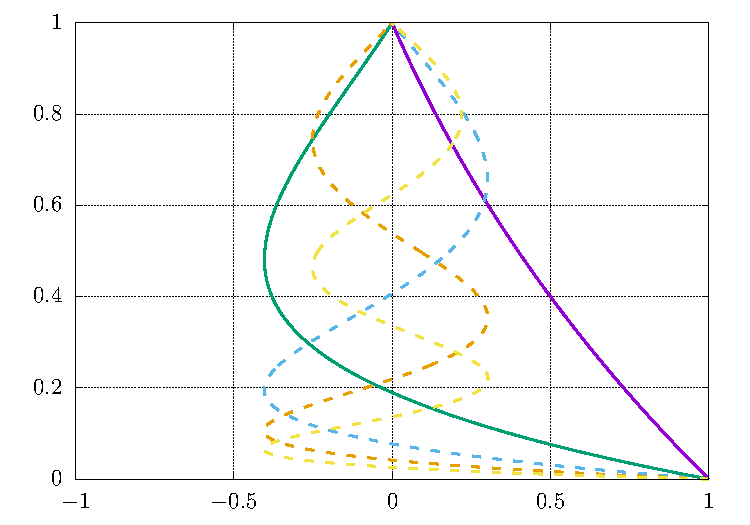
\includegraphics[width=0.8\textwidth]{Relatório/Figuras/CordaProblem.pdf}
    % \vfill
    % \usebeamerfont{title} Contato: \texttt{caiotomas6@gmail.com}
\end{frame}
%
\end{document}